\chapter{Learning from ideal data\\}
\label{cha:Learning_algorithm}

This chapter is focussing on the implementation of the inverse reinforcement learning idea that is explained at the end of chapter \ref{cha:Literature_study}. It will start with a detailed explanation and discussion of the simulations done in order to check what the algorithm is capable of. In this chapter an ideal situation is assumed which means that data is generated with the same vehicle model used to learn the weights and the assumption that the observations are generated as the solutions of a cost function similar to \ref{eq:1} is exactly fulfilled. Afterwards the step is made to use a more sophisticated 15 degrees of freedom vehicle model with the use of the Amesim software and it is checked how accurate results are learned when the assumption on the observations is violated. Next a new learning approach is proposed which is based on a fitting algorithm and makes use of taylor expansions. 

\section{Ideal learning situation }

\textbf{Deze sectie moet nog herschreven worden en nagekeken}

\subsection{Non-linear vehicle model}\label{sec:Vehicle_models}
In this paper the controller is designed on top of a nonlinear bicycle model \cite{TongDuySon2019} as can be seen in figure \ref{fig:bicycle_model}.\\

\begin{figure}[h!]
	\centering
	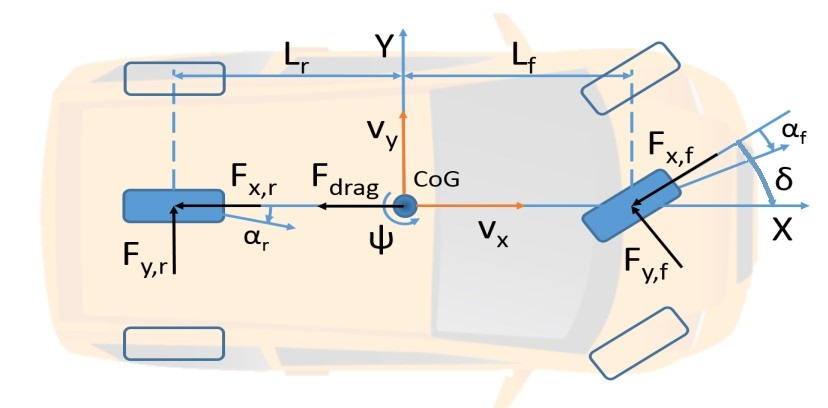
\includegraphics[width=0.5\textwidth]{Bicycle_model_paper.png}
	\caption{Non-linear vehicle bicycle model (Source: \cite{TongDuySon2019}).}
	\label{fig:bicycle_model}
\end{figure}

In this model, the vehicle system is characterised with 6 states and 2 inputs:
\begin{equation}\label{eq:bicycle_model}
\centering
\bm{x} = 
\begin{bmatrix}
X & Y & v_x & v_y & \psi & \dot{\psi}
\end{bmatrix}^{T}
\; and \; \bm{u} = 
\begin{bmatrix}
t_r & \delta
\end{bmatrix}^{T}
\end{equation}

In this formulation, $X$ and $Y$ are the position of the centre of the car in the global coordinate system (capital symbols). $\psi$ is the vehicle yaw angle and $\dot{\psi}$ the yaw angular velocity. $v_x$ and $v_y$ are the vehicle velocities in the local vehicle frame (small symbols). The input vector consists of the throttle control input $t_r$ and the steering angle $\delta$.\\

The equations of motion \cite{TongDuySon2019} are:
\begin{equation}\label{eq:bicycle_model_eqmotion}
\begin{aligned}
\dot{X} = v_x cos(\psi) - v_y sin(\psi)\\
\dot{Y} = v_x sin(\psi) + v_y cos(\psi)\\
\dot{\psi} = \dot{\psi}\\
m \dot{v}_x = F_{x,f} cos(\delta) - F_{y,f} sin(\delta) + F_{x,r} - F_{drag} + m v_y \dot{\psi}\\
m \dot{v}_y = F_{x,f} sin(\delta) + F_{y,f} cos(\delta) + F_{y,r} - m v_x \dot{\psi}\\
I_z \ddot{\psi} = L_f (F_{y,f} cos(\delta) + F_{x,f} sin(\delta)) - L_r F_{y,r}
\end{aligned}
\end{equation}

The used fixed parameters are the total vehicle mass $m$, the z-axis moment of inertia $I_z$ and the distances between the centre of gravity (COG) and the front and rear axle $L_f$ and $L_r$.\\

The drag force is calculated as:
\begin{equation}\label{eq:bicycle_Fdrag}
\begin{aligned}
F_{drag} = C_{r0} + C_{r1} v_x^2
\end{aligned}
\end{equation},
with $C_{r0}$ the roll resistance and $C_{r1}$ the air drag contributions.\\

To calculate the tyre forces, a linear tyre model is used. The longitudinal tyre forces are calculated as:
\begin{equation}\label{eq:bicycle_Fx}
\begin{aligned}
F_{x,f} = \frac{t_r T_{max}}{2 R_w}\\
F_{x,r} = F_{x, f}
\end{aligned}
\end{equation}

$R_w$ is the wheel radius and $T_{max}$ a measure for the maximum torque the engine is able to supply. In this way, four wheel drive is assumed and the total torque is equally distributed between front and rear axle (division by 2 in above equations). The coefficient $t_r$ is the normalised wheel torque and can have a value between -1 and 1 (negative for braking).
The lateral tyre forces are calculated based on the tyre slipangles $\alpha_f$ and $\alpha_r$:
\begin{equation}\label{eq:bicycle_slipangle}
\begin{aligned}
\alpha_f = -atan(\frac{\dot{\psi} L_f + v_y}{v_x}) + \delta\\
\alpha_r = atan(\frac{\dot{\psi} L_r - v_y}{v_x})
\end{aligned}
\end{equation},
resulting in:
\begin{equation}\label{eq:bicycle_Fy}
\begin{aligned}
F_{y,f} = 2 K_f \alpha_f\\
F_{y,r} = 2 K_r \alpha_r
\end{aligned}
\end{equation}\\
The use of this linearised lateral tyre model is valid for small lateral accelerations ($a_y <= 4 m/s^2$) and slip angles ($\alpha <= 5^o$) \cite{TongDuySon2019}. It is acceptable to use this model in this paper as the goal is to control a comfortable and thus smooth lane change manoeuvre. These constraints will also be checked during the validation.\\

The fixed model parameter used during the simulations are given in table \ref{table:vehicel_model_param}. These correspond to common used vehicle parameters as found in paper \cite{Yankov}.

\begin{table}[h]
	\centering
	\begin{tabular}{|p{5cm}|p{2cm}|}
		\hline
		\textbf{Parameter} & \textbf{Value}\\ \hline		
		Vehicle mass $m$ [kg] & 1430\\ \hline
		Moment of inertia $I_z$ [$kgm^2$] & 1300\\ \hline
		Front axle distance $L_f$ [m] & 1.056\\ \hline
		Rear axle distance $L_r$ [m] & 1.344\\ \hline
		Roll resistance coefficient $C_{r0}$ [N] & 0.6\\ \hline
		Air drag coefficient $C_{r1}$ [$\frac{Ns^2}{m^2}$] & 0.1\\ \hline
		Engine torque limit $T_{max}$ [Nm] & 584\\ \hline
		Wheel radius $R_w$ [m] & 0.292\\ \hline
		Lateral front tyre stiffness $K_{f}$ [N] & 41850.85\\ \hline
		Lateral rear tyre stiffness $K_{r}$ [N] & 51175.78\\ \hline
		
	\end{tabular}
	\caption{Used vehicle model parameters.}
	\label{table:vehicel_model_param}
\end{table}

\subsection{defining the problem}
\textbf{Kijk slides 31 maart na, problem definition helemaal op het einde nog verwerken in de tekst.}

The method applied in order to check the consistency of the learning algorithm is to generate data that are generated by solving the 











%Bespreek het vehicle model. Lees featueres stukje na dat geschreven heb voor taak VS. X en Y variables zijn in longitudinal axis. Maakt gebruik van een complexer model --> kromming van het pad zit al inherent in de normal acceleration van het voertuig. --> versnellingen die ik beschouw zijn de totale versnellingen. 
%
%%An overview of the flow of the algorithm can be seen in Figure blablabla. (Explain flow of code and make connections with the above explained theory behind the model.)
%
%De gevonden trajectories vergelijken met een standaard lane change uit de literatuur --> zie $lane_change_kin$ voor foto. \\
%
%Zeg dat eerst de appraoch was tested in ideale omstandigheden: zelfde voertuigmodel werd gebruikt en de assumptie dat de date is gegenereerd door de minimalizatie van een comfort kostfunctie werd aan voldaan. 
%
%
%Herinner de lezer nog even de structuur die gaat worden gevolgd. 
%Learning, planning, tracking, validatie.
%Dit hoofdstuk zal over de learning gaan.
%Hoe is algorithm opgebouwd? Wrm wordt dit zo gedaan?
%Welke vehicle modellen wordt er gebruikt? Wrm mag men hier een simple vehicle mode gebruiken?
%Dit is gemachtigd omdat men hier de omgeving wil scannen voor een feasible pad --> dit wordt trager gedaan dan de tracking.(tracking zal gebruik maken van een meer complex model) Path planning ligt focus vooral op de omgeving.
%Goed refereren naar het rapport en VS rapport
%Wat zijn de assumpties die werden genomen?
%
%Hoe zal de methode gevalideerd worden? Leg de twee methodes uit: code generatie en kijken of de wegings factoren terug gevonden kunnen worden? Mappen de feature values met de values van het geobserveerde pad? --> is het doel dat gevolgd probeert te worden haalbaar? 
%
%Ga hier niet meer te diep in op de entropie. Leg het hier meer intuitief uit om de lezer niet te verwaren. 
%
%Vermeld afleiding van algortihm. Leg uit in Thesis hoe komt aan gradient die gebruikt. Zie papers: Ziebart et al and Kretzschmar et al.
%
%Modeleer een andere bestuurder. Can try to reproduce a data set with a change of parameters which represents a different driver. Can check that the learned model is also different. Hiermee aantonen dat er ook echt andere wegingsfactoren worden gegenereerd en dat de specifieke driving characteristics worden meegenomen.
%
%Ligt een tipje van de sluier op : hoe zal de data gegenereerd worden? 
%Plot simulink model en duidt de blokken aan die zullen worden ingevuld. Hier gaat dieper in gegaan worden in de volgende hoofdstukken. 
%
%Maak een vermelding dat men het menselijke gedrag van het geleerde model kan nagaan met een Turing test.\\
%
%Maak een plotje zoals paper Learning to Predict Trajectories of Cooperatively Navigating Agents --> feature variance afwijking en average error. (zelfde plotjes als al de papers)\\
%
%Schrijf een paragraaf over hoe de data gegenereerd wordt. --> leg kort het gebruik van de verschillende vehicle modellen uit. 
%
%
%
%Schrijf een paragraaf over de theta update --> zie RPROP methode --> beschrijf wrm beter is dan andere methodes die gezien werden. Bespreek hoe de parameters werden gekozen. 
%
%
%Kan vermelding maken dat in deze thesis de features zijn gekozen met de hand --> men kan proberen om de features ook te leren van date (Characterizing Driving Styles with Deep Learning)
%
%\clearpage
%
%
%%Afleiding van exponentiël functie zie paper: Feature-based prediction of trajectories for socially compliant navigation (foto) --> weights are lagrange coefficients.


%\section{Tables}
%Tables are used to present data neatly arranged. A table is normally
%not a spreadsheet! Compare \tref{tab:wrong} en \tref{tab:ok}: which table do
%you prefer?
%
%\begin{table}
%  \centering
%  \begin{tabular}{||l|lr||} \hline
%    gnats     & gram      & \$13.65 \\ \cline{2-3}
%              & each      & .01 \\ \hline
%    gnu       & stuffed   & 92.50 \\ \cline{1-1} \cline{3-3}
%    emu       &           & 33.33 \\ \hline
%    armadillo & frozen    & 8.99 \\ \hline
%  \end{tabular}
%  \caption{A table with the wrong layout.}
%  \label{tab:wrong}
%\end{table}
%
%\begin{table}
%  \centering
%  \begin{tabular}{@{}llr@{}} \toprule
%    \multicolumn{2}{c}{Item} \\ \cmidrule(r){1-2}
%    Animal    & Description & Price (\$)\\ \midrule
%    Gnat      & per gram    & 13.65 \\
%              & each        & 0.01 \\
%    Gnu       & stuffed     & 92.50 \\
%    Emu       & stuffed     & 33.33 \\
%    Armadillo & frozen      & 8.99 \\ \bottomrule
%  \end{tabular}
%  \caption{A table with the correct layout.}
%  \label{tab:ok}
%\end{table}




%%% Local Variables: 
%%% mode: latex
%%% TeX-master: "thesis"
%%% End: 
